\documentclass{article}

\usepackage[letterpaper,top=2cm,bottom=2cm,left=3cm,right=3cm,marginparwidth=1.75cm]{geometry}
\usepackage{graphicx,subcaption,lipsum}
\graphicspath{ {./images/} }
\usepackage{float}
\usepackage[colorlinks=true, allcolors=blue]{hyperref}
\usepackage{listings}
\usepackage{color}
\usepackage{xparse}

\definecolor{dkgreen}{rgb}{0,0.6,0}
\definecolor{gray}{rgb}{0.5,0.5,0.5}
\definecolor{mauve}{rgb}{0.58,0,0.82}

\lstset{frame=tb,
	language=Bash,
	aboveskip=3mm,
	belowskip=3mm,
	showstringspaces=false,
	columns=flexible,
	basicstyle={\small\ttfamily},
	numbers=none,
	numberstyle=\tiny\color{gray},
	keywordstyle=\color{blue},
	commentstyle=\color{dkgreen},
	stringstyle=\color{mauve},
	breaklines=true,
	breakatwhitespace=true,
	tabsize=3
}

\title{
	Arquivos distribuídos\\
	\large Relatório de implementação do trabalho 2\\INE5645 - Programação Paralela e Distribuída.
}

\author{Giovane Pimentel de Sousa - 22202685\\
		Guilherme Henriques do Carmo - 22201630\\
		Isabela Vill de Aquino - 22201632
}

\begin{document}
\maketitle

\section*{Introdução}

O objetivo deste trabalho é a implementação de uma aplicação cliente/servidor distribuída utilizando sockets TCP para transferência de arquivos. A aplicação
simula operações comuns como as realizadas por comandos Unix, como `scp` e `cp`, mas com funcionalidades específicas, incluindo suporte para recomeço de
transferências interrompidas e controle de múltiplas conexões simultâneas. Adicionalmente, buscou-se aplicar conceitos de programação paralela e distribuída
para garantir a eficiência no processamento e atendimento de múltiplos clientes. Este relatório apresenta a arquitetura, os detalhes de implementação e as
decisões técnicas tomadas durante o desenvolvimento do sistema.

\section*{Como executar}

\subsection*{Servidor}
A compilação segue o formato básico de qualquer aplicação Go. A execução do servidor segue o formato de aplicações Unix:
\begin{lstlisting}
$ cd daemon && go build . # Este comando produzirá o binário remcp-serv.
$ ./remcp-serv daemon
\end{lstlisting}

Caso queira se saber qualquer saída mostrada pelo servidor como logs, conexões, erros em curso, etc., basta executar sem a flag daemon,
que o servidor será executado utilizando o terminal como standard output.

Com a flag \textbf{daemon} o servidor será executado como um daemon, também ficando disponível para aceitar conexões de clientes.

\subsection*{Cliente}
O cliente se comporta de maneira semelhante a comandos Unix como `scp` ou `cp`, interpretando o IP para determinar a direção da transferência. Exemplos de execução:
\begin{lstlisting}
$ cd remcp && go build . # Este comando produzirá o binário remcp.
$ ./remcp 127.0.0.1:/home/gio/Downloads/teste.txt /home/gio/arquivos_distribuidos/teste
$ ./remcp /home/gio/Downloads/teste.txt 127.0.0.1:/home/gio/arquivos_distribuidos/teste
\end{lstlisting}


- Caso o IP esteja no \textbf{primeiro} argumento, a transferência será \textbf{servidor => cliente}.

- Caso o IP esteja no \textbf{segundo} argumento, a transferência será \textbf{cliente => servidor}.

\section*{Implementação}

A implementação foi realizada em Go 1.23 e explorou várias técnicas e conceitos relevantes para sistemas distribuídos, incluindo:

\subsection*{Arquitetura}
A aplicação é dividida em dois componentes principais:

1. \textbf{Servidor (\textit{remcp-serv})}: Executa como um daemon, permitindo o atendimento simultâneo de múltiplos clientes, respeitando o limite máximo configurado.

2. \textbf{Cliente (\textit{remcp})}: Realiza transferências de arquivos, interpretando a direção com base nos argumentos fornecidos.

\subsection*{Configurações}
As principais configurações, como número máximo de conexões simultâneas e velocidade de transferência, estão implementadas como constantes no código.
Isso simplifica ajustes durante o desenvolvimento.

\begin{figure}[H]
	\centering
	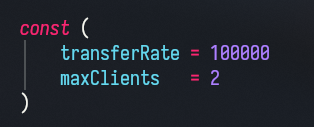
\includegraphics{constantes.png}
\end{figure}

Sendo:

- \lstinline{transferRate}: taxa transferência máxima, que eventualmente será dividida entre os clientes.

- \lstinline{maxClients}: o máximo de clientes que o servidor aceita simultâneamente.

\subsection*{Controle de concorrência}
Para garantir a integridade durante a execução paralela, mutexes foram utilizados nas regiões críticas. O servidor distribui a banda disponível
igualmente entre os clientes conectados, ajustando dinamicamente a velocidade de transferência.

\begin{figure}[H]
	\centering
	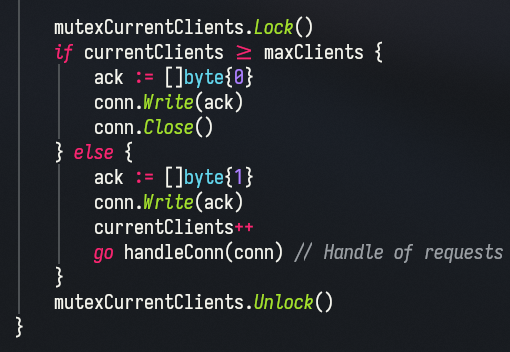
\includegraphics[scale=0.5]{concorrencia.png}
\end{figure}

\subsection*{Acknowledgments (ACKs)}
O uso de "acknowledgments" foi essencial para evitar problemas de mensagens malformadas. Sempre que uma mensagem é enviada entre cliente e servidor,
o receptor confirma o recebimento antes de prosseguir.

\begin{figure}[H]
	\centering
	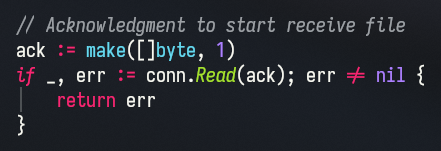
\includegraphics{acks.png}
\end{figure}


\subsection*{Mecanismo de retry}
Quando o número máximo de conexões é atingido, o cliente tenta se reconectar automaticamente ao servidor. O comportamento segue esta lógica:

- Até 5 tentativas são realizadas, com um intervalo de 5 segundos entre elas.

- Caso o limite persista, a conexão é encerrada com um erro.

\begin{figure}[H]
	\centering
	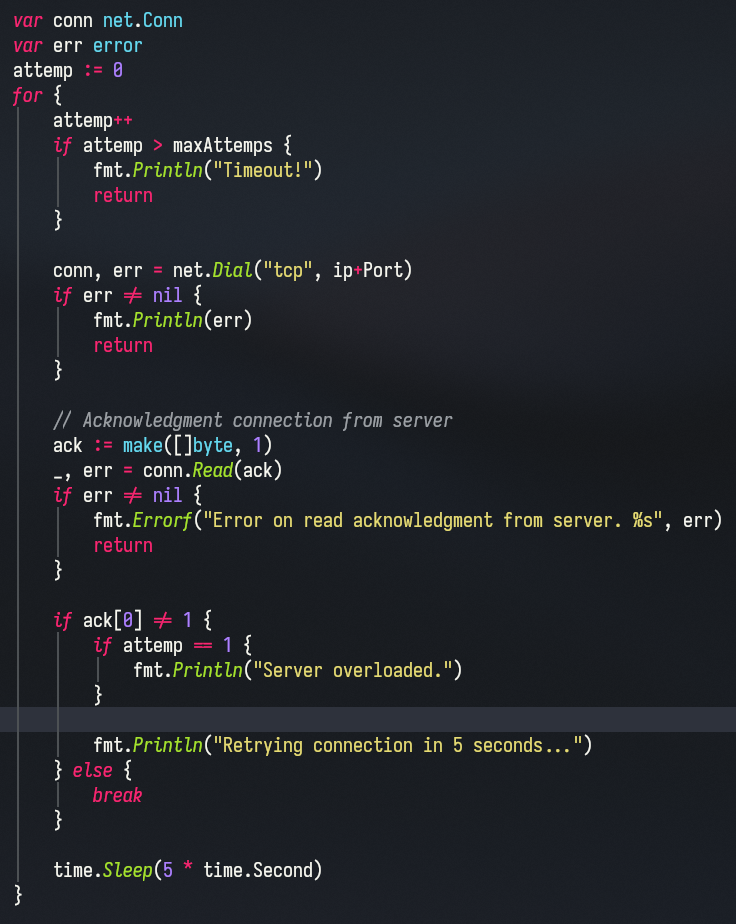
\includegraphics[scale=0.5]{retry.png}
\end{figure}

\subsection*{Recomeço de transferências}
Quando uma transferência é interrompida por qualquer circustância, elas podem ser retomadas da seguinte forma:

- Durante a inicialização de uma transferência, o cliente verifica a existência de arquivos \textit{.part} e informa ao servidor o ponto de recomeço. Assim
o servidor só precisa enviar o restante dos dados, não o todo.

\begin{figure}[H]
	\centering
	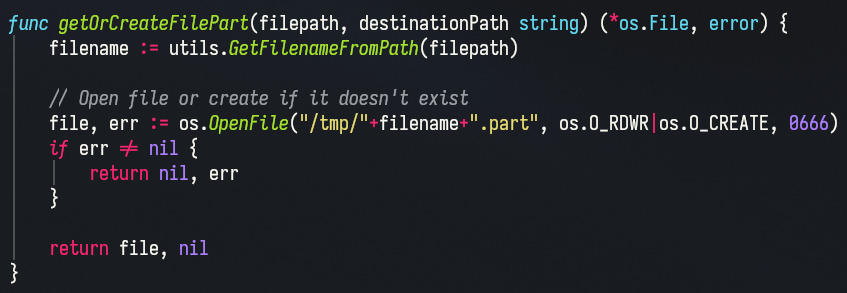
\includegraphics[scale=0.5]{part.png}
\end{figure}

- Arquivos parciais (\textit{.part}) são criados na pasta \textit{/tmp}, sendo ela utilizada como diretório padrão neste projeto. Quando a transferência
é finalizada, o arquivo é movido para o diretório inicialmente escolhido como destino, perdendo a extensão .part do seu nome.

\begin{figure}[H]
	\centering
	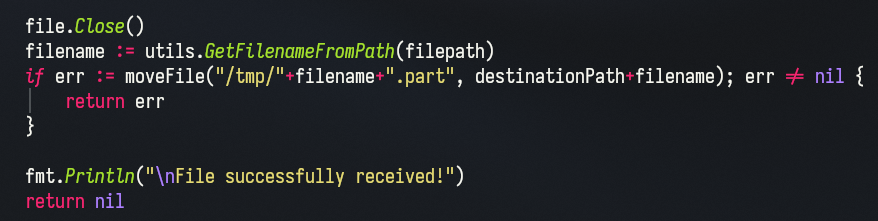
\includegraphics[scale=0.5]{move.png}
\end{figure}

\subsection*{Fluxo de transferências}
1. \textbf{Servidor => Cliente}: O cliente recebe os dados em partes, armazenando temporariamente até concluir o download.

2. \textbf{Cliente => Servidor}: A transferência ocorre de maneira direta, sem throttling ou controle adicional.

\begin{figure}[H]
	\centering
	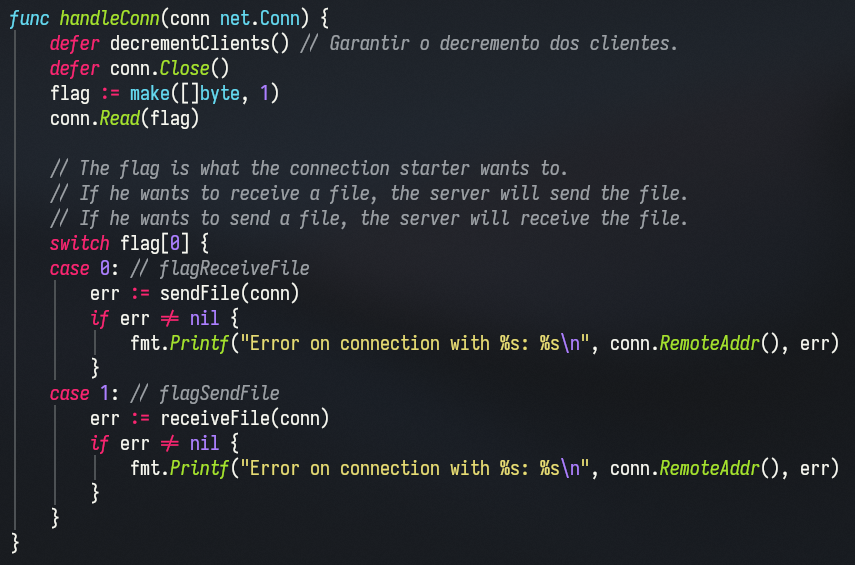
\includegraphics[scale=0.5]{flow-2.png}
	\caption{Controle de fluxo do Servidor}
\end{figure}

\begin{figure}[H]
	\centering
	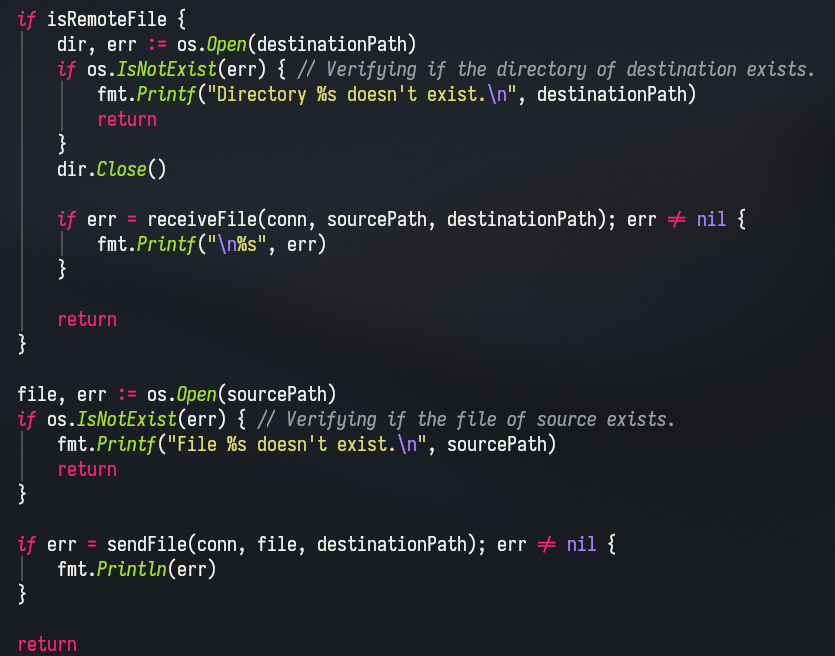
\includegraphics[scale=0.5]{flow-1.png}
	\caption{Controle de fluxo do Cliente}
\end{figure}

\section*{Parametrizações e testes}

Para validar o comportamento da aplicação em diferentes cenários, realizamos uma série de testes variando parâmetros como número máximo de conexões
simultâneas, velocidade de transferência e tamanhos dos arquivos enviados. Esses testes tiveram como objetivo assegurar a implementação correta
do sistema frente aos requisitos especificados.

Os testes para máximo de conexões foi menor pois como, no geral, o resultado é parecido, não se viu necessário tantos testes.

Foi validado como um servidor pode ficar sobrecarregado conforme muitas requisições/clientes chegam. Para resolver esse tipo de
problema, limitações de acesso são necessárias, evitando que o servidor se sobrecarregue, que é menos prejudicial do que não responder algumas requisições de
imediato.

\begin{figure}[H]
	\centering
	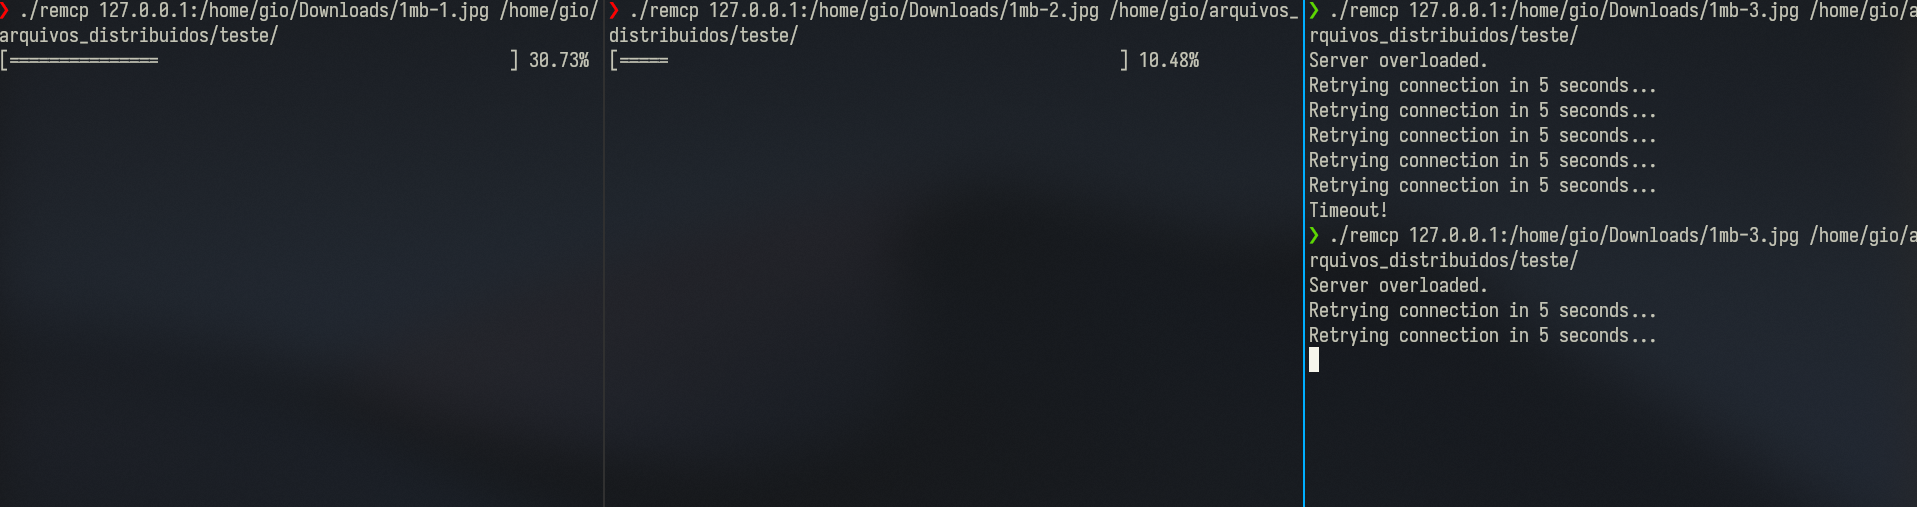
\includegraphics[width=0.98\textwidth]{run-1.png}
	\caption{Começo das transferências}
\end{figure}

Neste teste, configuramos o limite de conexões simultâneas no servidor para 2 clientes. Durante a execução, ao tentar estabelecer uma terceira conexão,
o servidor retornou um \textit{acknowledgment} de erro, e o cliente aguardou antes de realizar novas tentativas. Esse comportamento observado estava
conforme o esperado.

O arquivo de envio tinha o tamanho de 1MB, sendo transferido a uma taxa de 10.000 bytes por segundo.

\begin{figure}[H]
	\centering
	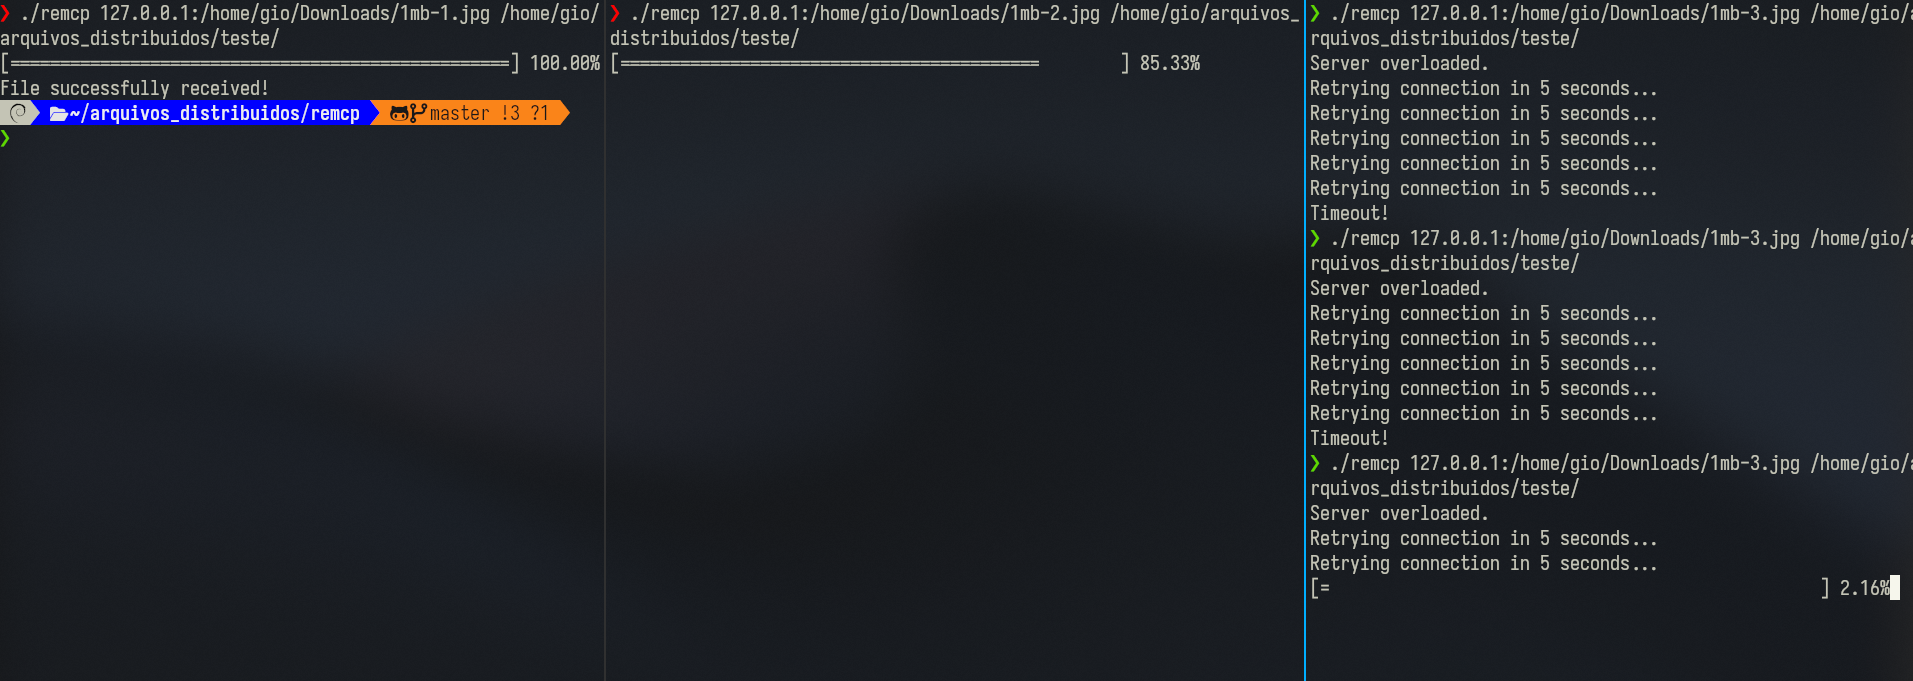
\includegraphics[width=0.98\textwidth]{run-2.png}
	\caption{Novas tentativas do cliente 3 de se conectar}
\end{figure}

Então, a transferência do cliente 1 finalizou e o cliente 3 enfim consegue se conectar com sucesso. Durante o tempo de espera para uma nova conexão por
parte do cliente 3 e a finalização de transferência do cliente 1, o cliente 2 obteve a banda de transferência toda para si, o que tornou, nem que seja
por pouco tempo, a velocidade de transferência mais rápida. Porém, sua felicidade durou pouco, pois com o mecanismo de retry, logo que foi possível,
a conexão foi estabelecidade entre o cliente 3 e o servidor, tendo agora a banda de transferência dividida entre estes dois clientes.

\begin{figure}[H]
	\centering
	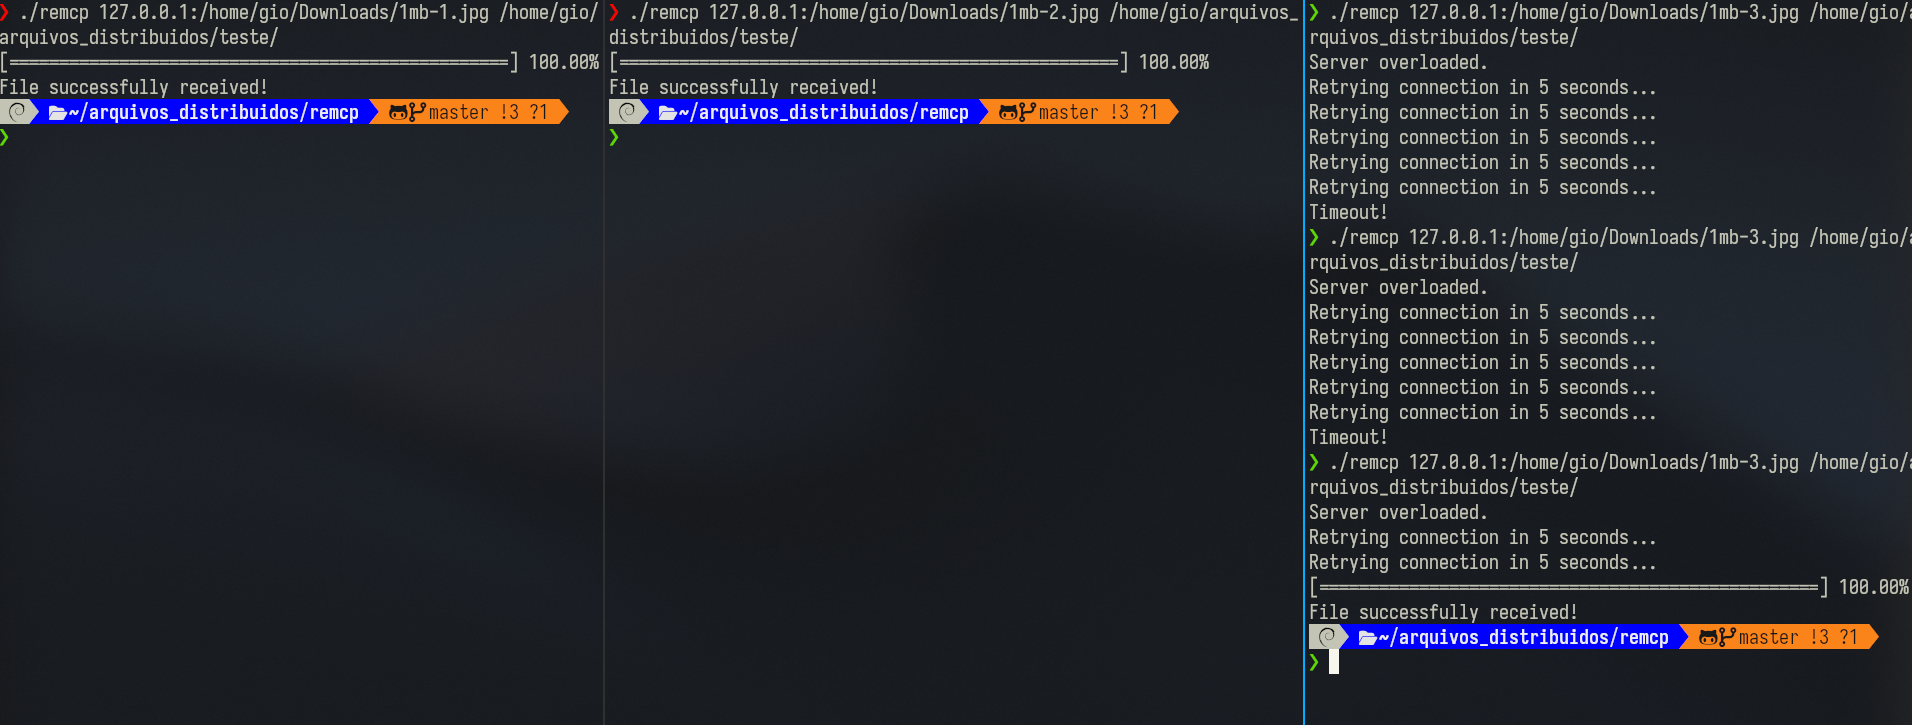
\includegraphics[width=0.98\textwidth]{run-3.png}
	\caption{Cliente 2 finaliza e cliente 3 fica com toda a taxa de transferência}
\end{figure}

Por fim, o cliente 2 finaliza, fazendo com que a banda de transferência fique toda para do cliente 3, tornando o envio do arquivo muito mais rápido em
comparação às outras duas transferências para o cliente 1 e o cliente 2.

\section*{Conclusões}

A implementação da aplicação cliente/servidor proposta atendeu integralmente aos objetivos do trabalho demonstrando a viabilidade de soluções distribuídas
para transferência de arquivos. O uso de sockets TCP, em conjunto com mecanismos como controle de concorrência e \textit{acknowledgments}, garantiu a
robustez e a funcionalidade esperadas.

Os desafios enfrentados ao longo do desenvolvimento estavam previstos no escopo do trabalho e foram abordados com as técnicas adequadas sugeridas. A divisão dinâmica
de banda, a limitação de conexões e o recomeço de transferências foram funcionalidades implementadas com sucesso e validadas em diferentes cenários de teste.

Embora a aplicação tenha cumprido os requisitos, melhorias futuras incluem a modularização de partes do código para facilitar manutenção e reutilização.
No entanto, as escolhas feitas durante o desenvolvimento permitiram uma solução eficiente e funcional, alinhada aos objetivos do trabalho.

\end{document}
